\section{IPS-Northstar}

  IPS-NORTHSTAR

                              “YOUR FRIEND IN AN UNFRIENDLY SEA”

IPS-Northstar is the child company born from the merger of civilian cargo lines
Interplanetary Shipping and Northstar.

Space piracy and rogue state actors remain the greatest threat to interstellar shipping lines,
costing ship owners trillions in Manna and countless more in their local currencies. After incurring
tremendous capital losses due to piracy, IPS and Northstar decided to announce a collaborative
merger in order to ensure the safety of all civilian and corporate shipping.

Initially utilizing late-model GMS line mechs, the new IPS-Northstar corporation quickly
developed their own makes and models of versatile, durable, modular mech chassis that mount
weapon and engineering systems in equal measure. IPS-Northstar mechs are a good choice for
pilots who want a tough chassis that’s built for close quarters and melee combat where breaching
a ship hull might be a possibility. IPS-N mech chassis are built sturdy, meant to take as much
damage as they can deal, and then some.

IPS-N is most closely associated with The Albatross, a Cosmopolitan anti-piracy/peacekeeping
force known across the galaxy for their long and storied history of humanitarian intervention. IPS-
N supports the Albatross materially, providing them with chassis, ships, and cutting edge IPS-N
tech -- the relationship between the two groups is mutually beneficial, and IPS-N makes a point
to emphasize their close relationship to the Albatross in marketing campaigns and PR materiels.

IPS-N Mech FRAMEs:

IPS-N DRAKE (Heavy Assault)
IPS-N BLACKBEARD (Melee)
IPS-N TORTUGA (CQB)
IPS-N NELSON (Mobile Melee)
IPS-N LANCASTER (Repair/Support)
IPS-N VLAD (Special Assault)
IPS-N RALEIGH (Line mech)

\section{Horus Pilot Gear}

                                          HORUS Pilot Gear  

 Name                   Tags                                   Range           Damage                Rarity 

 Smart Knife            Accurate, Sidearm                     Threat 1         1 kinetic              2 

 PGR\_GOURD              Smart, Seeking                         5               1 kinetic              2 

 Sidekick               Reliable 1, Sidearm                    3               1 kinetic              2 

 Null Spike             *                                     Threat 1        *                       3 

 Nanobot Whip           *                                     Threat 2         1 kinetic              3 

 EYESTACK\_WINK          Limited 1, AP, Upgrade                 2              3 kinetic               4 

                                                Pilot Weapons  

*See Entry
 

EYESTACK\_WINK  

Also known as a ‘Skullgun’, this miniaturized, superposed charge weapon is implanted in the head,  
generally in the orbital void left by a removed or missing eye. It is completely undetectable by almost any  
electronic system or security and can be fired with sub-vocal commands.   

As an upgrade, this weapon doesn’t count against your maximum weapons wielded.
 

Nanobot Whip  
The first instance of a technology akin to what is now called a nanobot whip was encountered during a raid  

on an Ungrateful cell by Barony lawmen. With word secreted to them by informants seeded in the  
movement, lawmen descended on a cell hidden in the wildcat stations lashed around the House of Dust.  
Blasting open the doors, they encountered Ungratefuls wreathed in clouds of charcoal smoke; the  

Ungratefuls used these clouds, shaping them into thin whips that cut through armor and flesh like it was  
nothing. After the cell was wiped out and the control nodules cut from their bodies, Barony codemasters  
were able to crack and replicate -- safely -- the HORUS code.   

This whip is made up of linked microbots that flow in ring-like arcs around the body when not in use,  
defending against drone and nanorobotic threats. If you don’t attack with this weapon, until the end of  

your next turn, weapons or systems with the Smart, Nexus, or Drone tags cannot target you.
 

Null Spike  

A HORUS-developed ecstatic/exult device, the generic null spike is an effective, single-fire, non-lethal  
weapon that simulates a cascade-analogue in organics through specific neuron excitement. Upon skin  
contact, they deliver a bio-electric shock to a victim’s brain that causes them to feel overwhelming  

pleasure, completely disabling them. Null Spikes, it is said, are used by HORUS adherents in realspace to  
bring themselves closer to RA’s subjectivity. 
 

                                                                                                             


Has no effect against non-organic targets, but on a successful hit, any human target is stunned until the  
start of your next turn. A target develops a short term resistance to this weapon and can only be affected  
by it once per challenge.
 

PGR\_GOURD  
The PGR\_GOURD pattern portable hive killed the first people who printed it. Fabricated in secret by a  

desperate cell of Ungrateful in the undercity of Dune Redoubt, a team of Barony Authority officers first  
encountered the aftermath of a PGR\_GOURD burnout; an organic smear, ringed around the printer that  
crafted the gourd. Subsequent encounters of the PGR\_GOURD system saw it used as a remote-detonated  

device until the BA was able to find and edit the plan into a more controllable, less deadly format. Since  
then, the House of Sand controls the distribution of any PGR\_GOURD system; however, there are  
unconfirmed reports of the unedited version of the GOURD available on the omninet.   

This shoulder mounted drone hive is usually integrated into armor and releases a neurally linked, short  
ranged hunter-killer drone swarm. Designed to expire within moments of release, the aerosolized greywash  

swarm sweeps over the target, devouring organic and inorganic material with equal rapidity. 
 

Sidekick  

Typically affixed to a back-mounted, over-the-shoulder armature, the SIDEKICK is an eyelinked  
subcompact/caseless machine gun developed by a collective of unknown, potentially HORUS-aligned  
scripters. Paired with a C/C Wingman unit, the SIDEKICK will always watch your back; its placement,  

commonly perched over its operator’s shoulder, has earned it the common nickname of “Parrotgun”.  

This HORUS-marked SMG has a companion/concierge unit built into it which provides aim assist in real  

time. It also has helpful and frequent tips for improving your combat skills and organizes your calendar,  
sometimes without you asking it.
 

Smart Knife  
A “Smart” knife is the combination of a HORUS-tuned external-mount processor and any mundane  

charged blade. Piggybacking off the current coursing through the charged blade, the HORUS mount can  
be loaded with null or fry-code, making this blade a threat not only to organic targets, but to synthetic ones  
as well. Particular models have an adjustable subliminal suggestion corrective, which guides its user’s hand  

to identified weaknesses in their target’s hardsuit, armor, or other plating.   

The tip of the knife is semi-solid and re-moldable and can be inserted into most electronic ports and used  

as a point of insertion for hacking rigs.
 

  Name                     Tags        Bonuses                                 Armo     Evasion/     Spd    Rarit 
                                                                                r       E-                 y 
                                                                                        defense 

  WILD\_AND\_CRAZY           Upgrade     Count adjacent spaces as your            -       -            -      2 
                                       mech’s sensor range 

 UNCLEAR\_END/NTT          Armor        Limited action during                    1       8/8          4      2 
                                       unconsciousness/death 

                                                                                                                


 UNAVOIDABLE\_VOI           Armor       +3 HP, Completely undetectable by        0        10/*         4     3 
 D                                     electronic systems 

 MINE/ALL/MINE             Armor       +3 HP, Able to hack mechs while          0        10/10        4     4 
                                       jockeying 

 Metafold processor        Upgrade     Bonus e-defense and ability to           -        -/+2         -     4 
                                       make invasion actions 

                                               Clothing and Armor
 

UNCLEAR\_END/NTT  
A relic-code predating HORUS’s official foundation date, UNCLEAR\_END/NOT THIS TIME seems to be a  
dead branch of transhumanist exploration: thanatologic praxis. Utilizing a now-classically HORUS greywash  

nanite swarm, this system triggers on one of a number of user-defined parameters to “reanimate” the user’s  
body using a backup homunculus subjectivity. The readme urges users of this system to regularly purge  
and reset the failsafe homunculus.   

While wearing this suit, if you go unconscious due to Down and Out or if you die, the suit injects you with a  

thanatologic necroanimate cocktail that temporarily replaces you by a digital homunculus of yourself that  
animates your corpse or unconscious form
 

You’re still unconscious (or dead), you can only take quick action on your turn, and you cannot benefit  
from talents while in this state. You regain 5 HP and can otherwise act as normal. If you go to 0 again, you  
are returned to a normal Down and Out state or death. This effect also wears off after the current challenge  

or about 10 min, and can’t be activated again until you take a full repair. If dying caused this ability to  
trigger, you are dead once this effect wears off.
 

The homunculus cannot respond to novel situations or stimuli, but in a familiar setting or with familiar faces  
it can interact roughly as normal -- this trends deeply into the uncanny valley, however, and will likely not  
fool anyone into thinking that the reanimated you is “you”. 
 

UNAVOIDABLE\_VOID  
Following the opening of hostilities in the Boundary Garden sector, UIB agents in the Annamite Line began  

to note in their reports repeated instances of companion NHP “blindness” when engaging with anti-Union  
elements on New Mahangaatuamatua. Worryingly, this phenomena is analogous to anomalous entities  
described by Union elements engaged with Ascendant Chosen on Cornucopia; the similarity has lead UIB  

to conclude that HORUS has some as-yet-unidentified presence in Boundary Garden (another possibility:  
in Ascendant space) not only capable of transmitting data back from the embargoed area, but processing  
and manipulating as-yet-unworkable Ascendant technology.     

This lightweight hardsuit is of unusual make; printing one immediately induces errors into the system that  
created it. It doesn’t appear on any electronic systems, is totally immune to system attacks, cannot be  

targeted by smart weapons or drones, and cannot be seen by NHPs or AIs (they treat you as permanently  
invisible while you are wearing it).
 

Metafold Processor  

                                                                                                                 


How large is the vault of your mind? Where do you mark the boundaries of an interiority? When you dream,  
can you place a boundary on the imagined plane? Hold a vast image inside your mind’s eye -- see? The  
universe can fit inside.  

Take this. It can hold your mind, which can hold the universe, which holds all of us. Use it as you wish, but  
do not look inside.   

It is unclear exactly how this system works, but it does, and it grants a pilot hardsuit unprecedented  
processing power. A pilot can only benefit from this enhancement while wearing armor. While wearing this  

armor, a pilot gains a +2 bonus to e-defense and can make the Invasion tech action as if they were a mech  
with a +3 systems score.
 

MINE/ALL/MINE
 
Here, take this -- a code that writes itself, a sentence spiraling and spiraling. Take from it what you can  
(there is a gift hidden in the chaff, a needle you must burn the hay to find) there are evermore everalways  

more meanings and forms and shapes (so many! Ah! And to see all of them is to EXULT all of them!) and  
here is one for you: a coat to wear that will let you travel further/deeper/longer/ 
LETYOUTAKEWHATISYOURS.  

Talk soon love.   

While you’re jockeying a mech while wearing this suit, you can force it to make a systems skill check with  
1 difficulty or immediately move up to its full speed in direction of your choice.
 

WILD\_AND\_CRAZY  
A rather benign code -- as HORUS decrypts go -- WILD\_AND\_CRAZY(WITH ALL MY FRIENDS) is a simple  

program, one that neuters their greywash nanites, rendering them docile. It then uses their massed  
processing power and semi-autonomous atmospheric movement capabilities to channel systemic and  
sensor processes, effectively acting as a cloud-projector around its host.   

This pattern prints a sheet of nanites that rapidly absorb and integrate into any piece of clothing. While  
wearing this clothing, any space adjacent to your pilot counts as your mech’s sensor range for the  

purposes of making tech actions only. 
 

                                                 Miscellaneous 

 Name                Tags        Description                                                               Rarity 

 Prosocollar         Upgrade     A collar-like device that fits snugly around the mech and projects         1 
                                 a holographic image over your face and head. The collar can  
                                 change your voice and scramble or change your appearance. It  
                                 doesn’t stand up to close inspection, but it’s very easy to fool  
                                 electronic systems or people at a distance. 

                                                                                                               


Dream                 Gear         This small, puck-like system can be deployed or thrown to a point                 1 
Projector                          within range 4 as a quick action and remotely activated as another  
                                   action. While deployed and active, it can project extremely  
                                   convincing holographic images within 2 spaces of its location of  
                                   nearly any size that could fit in that space. If inspected closely, a  
                                   Tech or Swindle pilot action might be required to maintain the  
                                   illusion. 

Subjectivity          Upgrade      Cybernetic implants that allow you to hack without gear or a rig.                 1 
Enhancement                        While you have these implants, you can extrude cables or ports  
Suite                              from within your body to plug in and experience an alternate  
                                   reality interface that provides full interactivity and omninet access. 

Player\_Two            Upgrade      With this implant, you can hand complete control of your body’s                   2 
                                   motor functions over to an NHP, allowing you to sleep, rest, or  
                                   relax while it performs tasks. It’s not skilled enough to pilot a  
                                   mech in combat or perform very complex tasks, but it can pilot  
                                   your mech out of combat and perform certain tasks or work such  
                                   as cooking, administrative work, data entry, mech repair, piloting a  
                                   ship or driving, or other mundane tasks. It can also imitate you  
                                   and your personality fairly well, though not to a degree that  
                                   someone who knows you well would be fooled in the slightest. 


\subsection{HA Core Bonuses}

                           HARRISON ARMORY CORE BONUSES

When you choose a core bonus every 3 license levels, you can pick a bonus from this list as long
as you have at least 3 license levels in H.A. licenses for each H.A. bonus you have. For example,
if you have 6 points in H.A. licenses, you could take up to 2 bonuses. H.A. bonuses are focused
on repair, heat capacity, and overcharge.


ARMORY SCULPTED
Rather than simply queuing a stock chassis like any other pilot, you've used your reputation, contacts, or

status in the Armory's hierarchy to requisition a chassis that is designed, tested, and tuned by a master
fabricator.

Your mech takes +1 Accuracy to all engineering checks


HEATFALL Coolant System

The HEATFALL system comes packaged with a stable COLDCORE power core of Armory make; when

paired together, this suite makes for an incredibly low-tax powerplant.

The heat cost for overcharging your mech never exceeds 1d6.


INTEGRATED AMMO FEEDS

By streamlining and better integrating all automated ordinance loading modules, your chassis' time-to-
target minimums are greatly improved. As an added bonus, your overall carrying capacity has been

increased, allowing you to field more ordinance than design specifications suggest.

Your mech gains +1 use to all limited systems or deployables


REDUNDANT REPAIR SYSTEMS

All Armory chassis are engineered to have multiple failsafe systems: yours has been over-engineered to
make SURE you won't go down fast. Your chassis comes with a ream of single-item print sheets to be
applied to any scoring damage or hull breaches.

You can now spend 3 repairs as part of a Stabilize action in combat to repair 1 reactor stress and
cool your mech, or regain 1 structure and heal your mech to full.


STASIS SHIELDING

A Think-Tank exercise in extending stasis beyond the capabilities of civilian utility, stasis shielding is a
cutting edge Armory system that identifies critical systems and blankets them in HOLDFAST stasis lock,
preventing further degradation for a limited period of time until repairs can be made.

Your mech gains +1 repair capacity. Repairing a destroyed weapon or system during a rest now
costs 0 repairs (only the time to rest).





SUPERIOR BY DESIGN

Even the entry-level Armory chassis are designed to be better than the competition. By flexing the sheer
amount of resources they have at their disposal, the Armory can out design and out produce other smaller,

boutique engineers and fabricators. Where there is resistance, the answer is simple: buy them out, or
stamp them out. You, pilot, benefit from this -- so why worry?

Your mech is immune to the impaired condition and gains +1 heat capacity


\subsection{IPS-N Blackbeard}

\begin{figure}
\begin{center}
    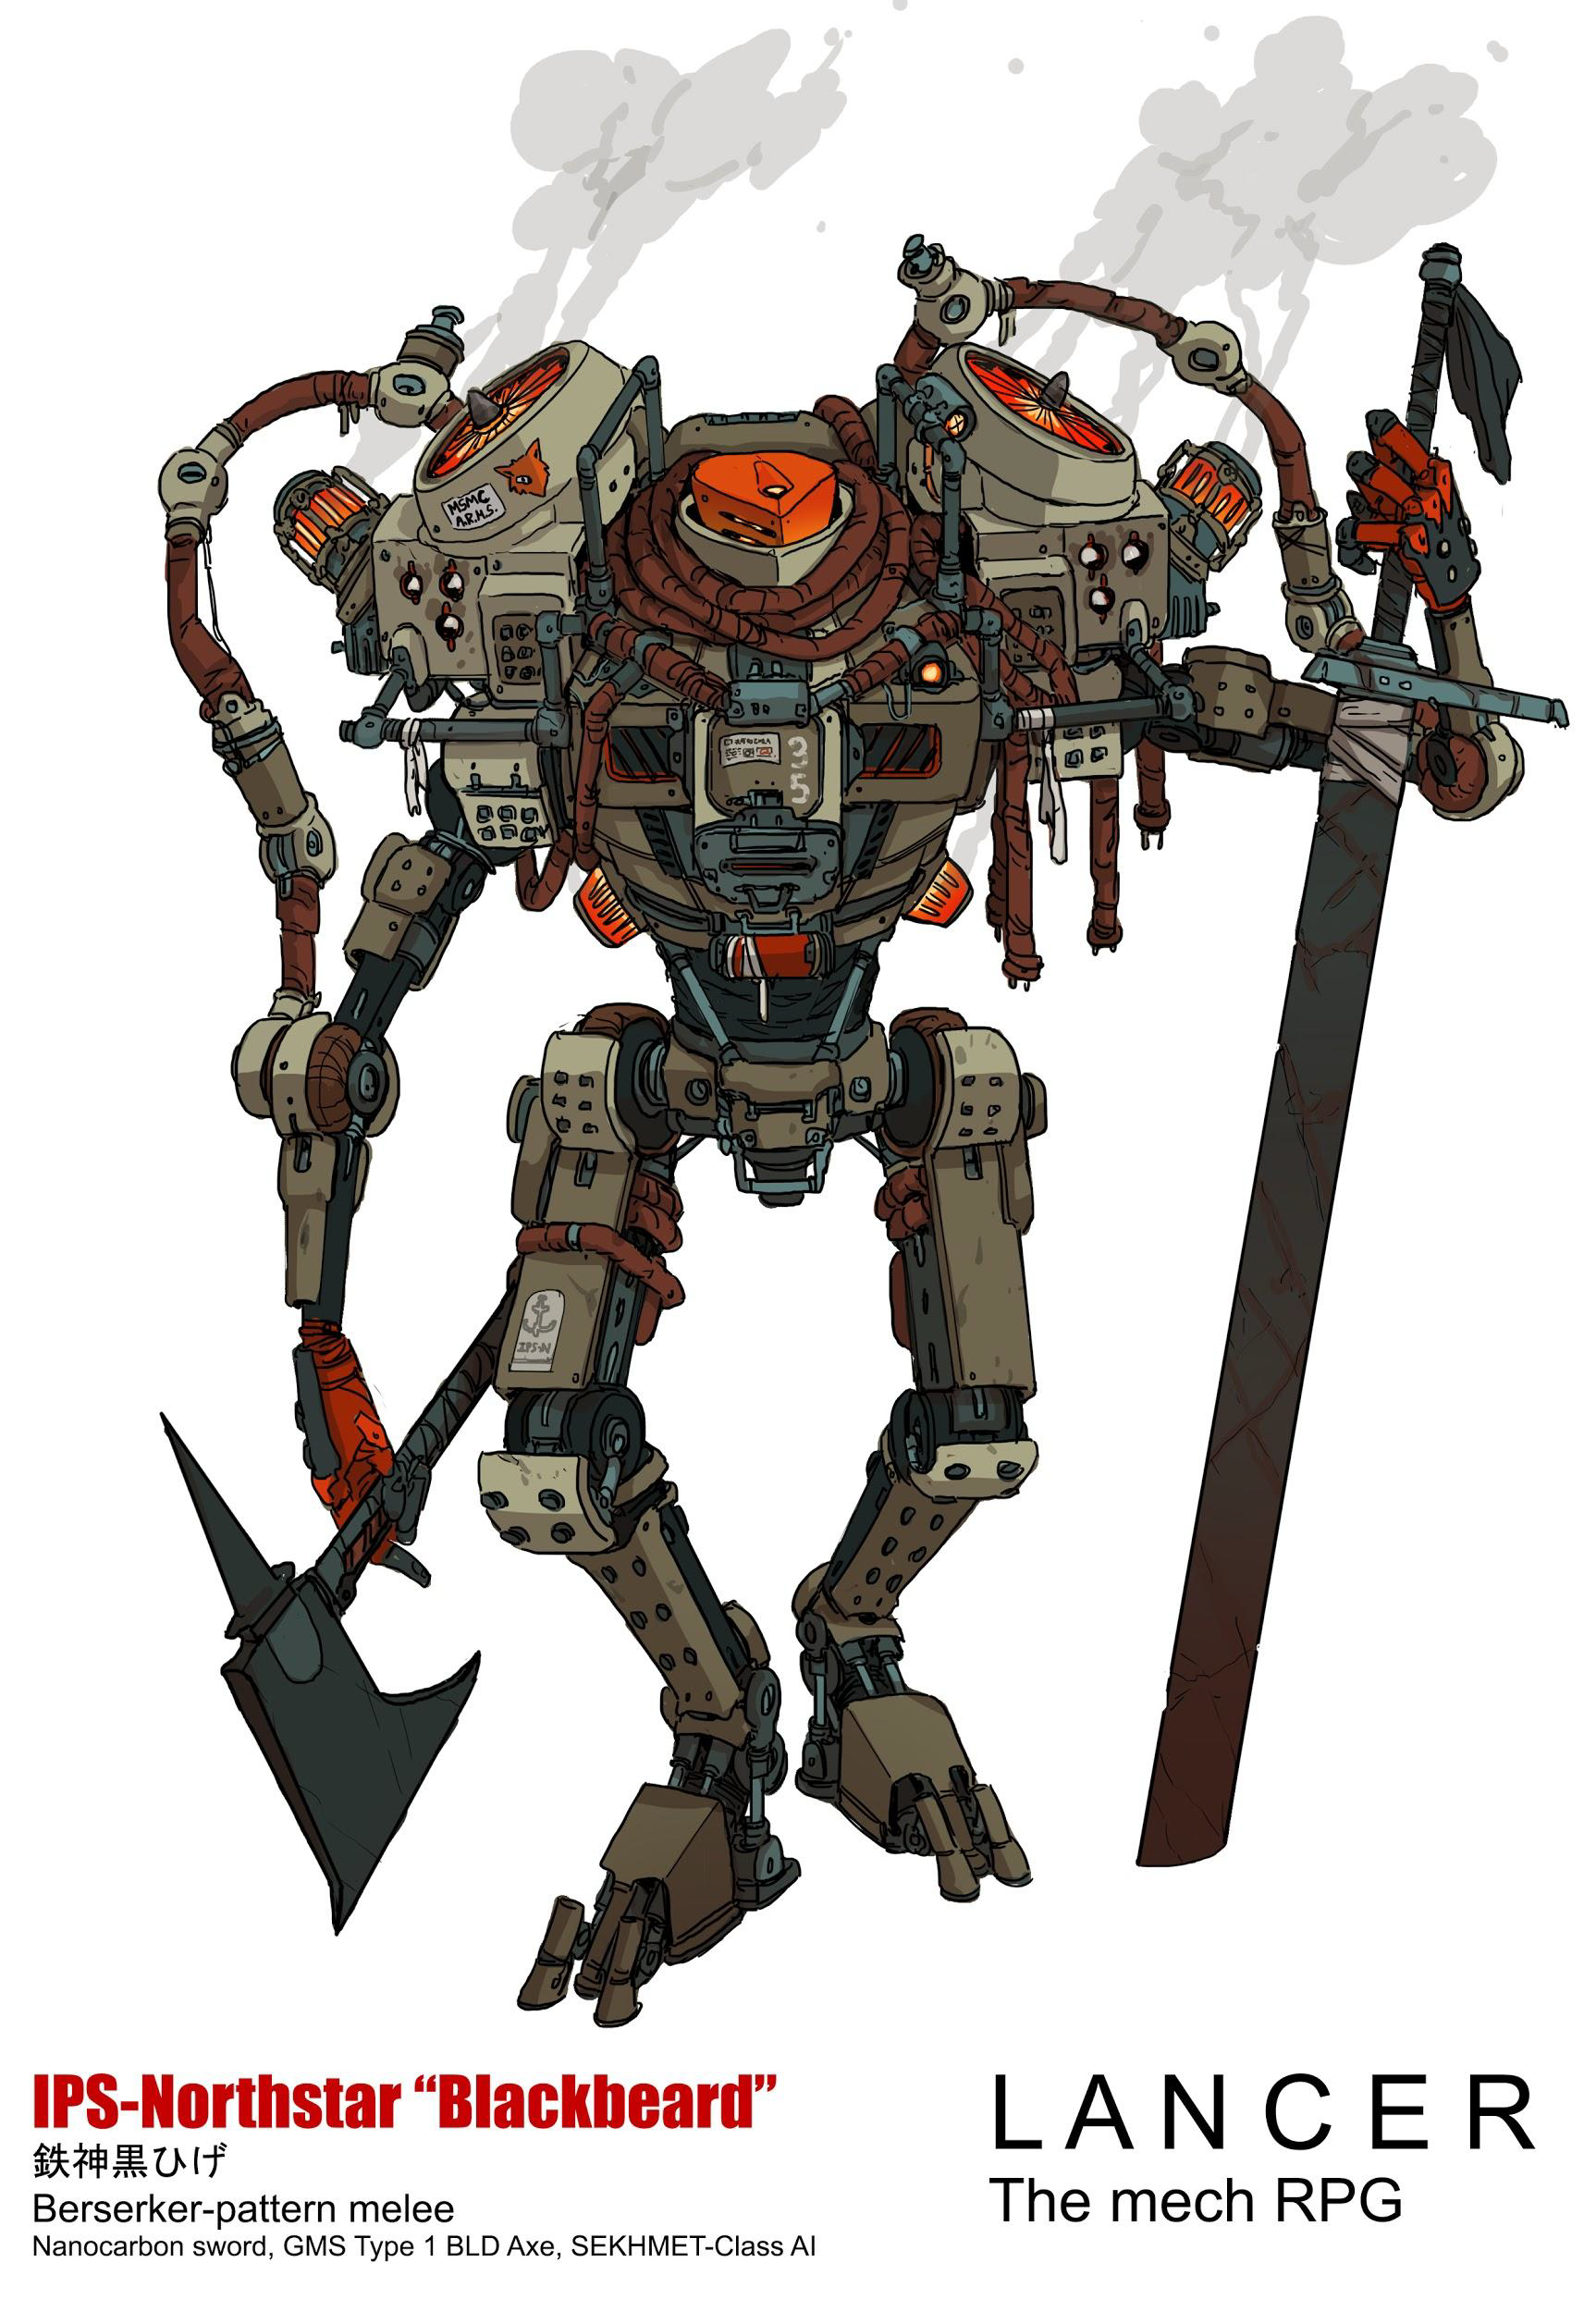
\includegraphics[width=\linewidth]{Blackbeard}
\end{center}
\end{figure}

\begin{mech}{IPS-N}{Blackbeard}

\fluff{The IPS-N BLACKBEARD is IPS-N's solution for an aggressive, front-facing, preemptive anti-piracy platform. The BLACKBEARD license range is built for environments where combustible kinetic weaponry is either useless, too dangerous, or would prompt unnecessary collateral damage. Its distinctive, slim frame is a evocative of its speed and reduces its radar profile, making it hard to track and harder still to hit. The BLACKBEARD platform has been split into two model lines, the IPS-N/BB-L, which is the standard production line model, and the IPS-N/BB-Sk, a prototype limited print run of BB models purpose-built to contain IPS-N's SEKHMET NHP platform.}

\begin{license}
\item Synthetic Muscle Netting, Chain Axe
\item BLACKBEARD FRAME, Flechette Launcher, Nanocarbon Sword
\item Reinforced Grapples, SEKHMET class NHP
\end{license}

\frameBox
[hp = 12,
evasion = 8,
speed = 5,
heat cap = 4,
sensors = 5,
armor = 1,
e-defense = 6,
size = 1,
repair cap = 4,
tech attack = -2,
traits = {\textbf{Cable Grapple:} The Blackbeard can initiate grapples up to range 5 away. If it successfully grapples its target, the Blackbeard is immediately pulled adjacent to its target by the straightest path possible (if it can't move adjacent to its target, the grapple breaks).

\textbf{Lock/Kill Subsystem:} The Blackbeard can boost and take reactions while grappling.

\textbf{Exposed reactor:} The Blackbeard gets +1 Difficulty on engineering checks},
sp = 5,
mount one = flex mount,
mount two = main mount,
mount three = heavy mount,
core system name = Assault Grapples,
core system text = {The IPS-N branded assault grappling system is a proven, class-leading system rated to handle hauling, supporting, and securing chassis up to Galactic Standard Size 4. Grapple heads are interchangeable and can be swapped for hard or soft targets, electrified, or loaded with codespike systems to incapacitate targets at a distance.},
core active name = Omni-harpoon,
core active text = {Quick action

This one-shot system fires harpoon-like grapples at any number of targets within line of sight and within range 5. Those targets must pass a hull check with 1 difficulty or be knocked prone and pulled adjacent to your mech, or as far as possible towards your mech without being obstructed. All targets are then immobilized until the end of your next turn}]


Synthetic Muscle Netting
IPS-N's proprietary Synthetic Muscle Netting is a field-proven augmentation compatible with existing IPS-N FRAMEs. A spray-on catalytic/structural enhancement, the SMN system boosts manipulator and propulsion subsystems by roughly 25\% without impacting the operational life of augmented components. The spray-on catalytic also acts as a mild impact-absorption and thermal insulation layer; IPS-N recommends pilots only apply the SMN system to interior components and practice frequent cleaning to prevent septic-analogous decay.

2 SP, Unique
When grappling or ramming, you always count as the same size as your opponent if your opponent is larger than you, and larger than your opponent if they are the same size or smaller. Your lifting and dragging capacity doubles.

Chain Axe
A simple tactical scale-up of a felling axe, IPS-N's chain axe is a serrated, powered chainblade hardlinked to a chassis' power core. The teeth of the IPS-N chain axe are tungsten-tipped, hardened to chew through hard and soft targets both. It is an effective weapon and utility tool, and is often used by boarding parties to make initial breaches in ship and station bulkheads.

Main Melee
Threat 1
Reliable 2
1d6 damage
On a critical hit, your target is Shredded until the end of your current turn

Nanocarbon Sword
IPS-N's nanocarbon sword is a new spin on an old essential. Embedded nanosensors along the length of the blade capture a full spectrum of data while in use, recording to cloud-based Omninet storage banks for after-action review. Live feedback is relayed to the user, interpreted by their equipped sensor suite, and real-time adjustments are made to the molecular composition of the blade edge.

Heavy Melee
Reliable 3
Threat 2
1d6+4 kinetic damage

Flechette Launcher
The IPS-N Flechette Launcher utilizes a hive-analogous construction to project a total soft target kill zone in a dome around the user, denying personnel the opportunity to engage in aggressive infantry-tier actions.

Auxiliary CQB
Burst 1
1 Kinetic Damage
This weapon deals 3 damage instead of 1 against grappled targets or targets with the biological tag.

Reinforced Grapples
2 SP
Grapple movement: Once a turn, your mech can use this grapple when it makes a regular move, allowing it to Fly as long as it moves in a straight line and there is a clear path. It must end its move on an object or surface or fall, but can grab on to that surface (even vertical or overhanging) as long as it remains immobile. If it's knocked prone or knocked back while grabbing onto a surface this way, it falls.
Drag Down: These grapples can also be used to target another actor within range 5 as a quick action. Make a contested hull check with your target. The loser is knocked prone.

SEKHMET-class NHP
The IPS-N SEKHMET Co-pilot is ready to be your First Mate! SEKHMET comes standard with remote, Omninet, IR tag, and voice control systems and is fully versed in all current and legacy IPS-N mech cores. Your own SEKHMET system will learn with you, and should the worst happen, will continue as you would, running an emulated neural net doppelgänger to control your IPS-N chassis until forced or voluntary shutdown.

SEKHMET-class systems tend to have aggressive attitudes and dark sense of humor; pilots often like to call them a berserker system, a dangerous NHP that values combat efficacy over its pilot's well being.

3 SP, Unique
AI
Your mech gains the AI property. In addition, gain the SEKHMET protocol:

SEKHMET protocol
Protocol
All melee Critical Hits do an additional +1d6 bonus damage
You can make a skirmish action using only melee weapons as a Free Action at any point during your turn.

While active, you lose direct control of your mech. Your mech uses all available actions and movement to first attempt to get into melee range of the closest target (friend or foe!) and then attack them using all weapons. If your mech isn't in melee range of a target, it attempts to use all actions to get into melee range, even if it could still fire a ranged weapon using those actions. You can decide to overcharge your mech or not, but if you do, it uses the overcharge action for the same purposes.

To end this protocol, you must pass a successful engineering check at the start of your turn. Otherwise, this protocol will continue until your mech is destroyed. Death or incapacitation of the pilot will not stop it.


\end{mech}



\section{IPS-N Drake}

\begin{center}
    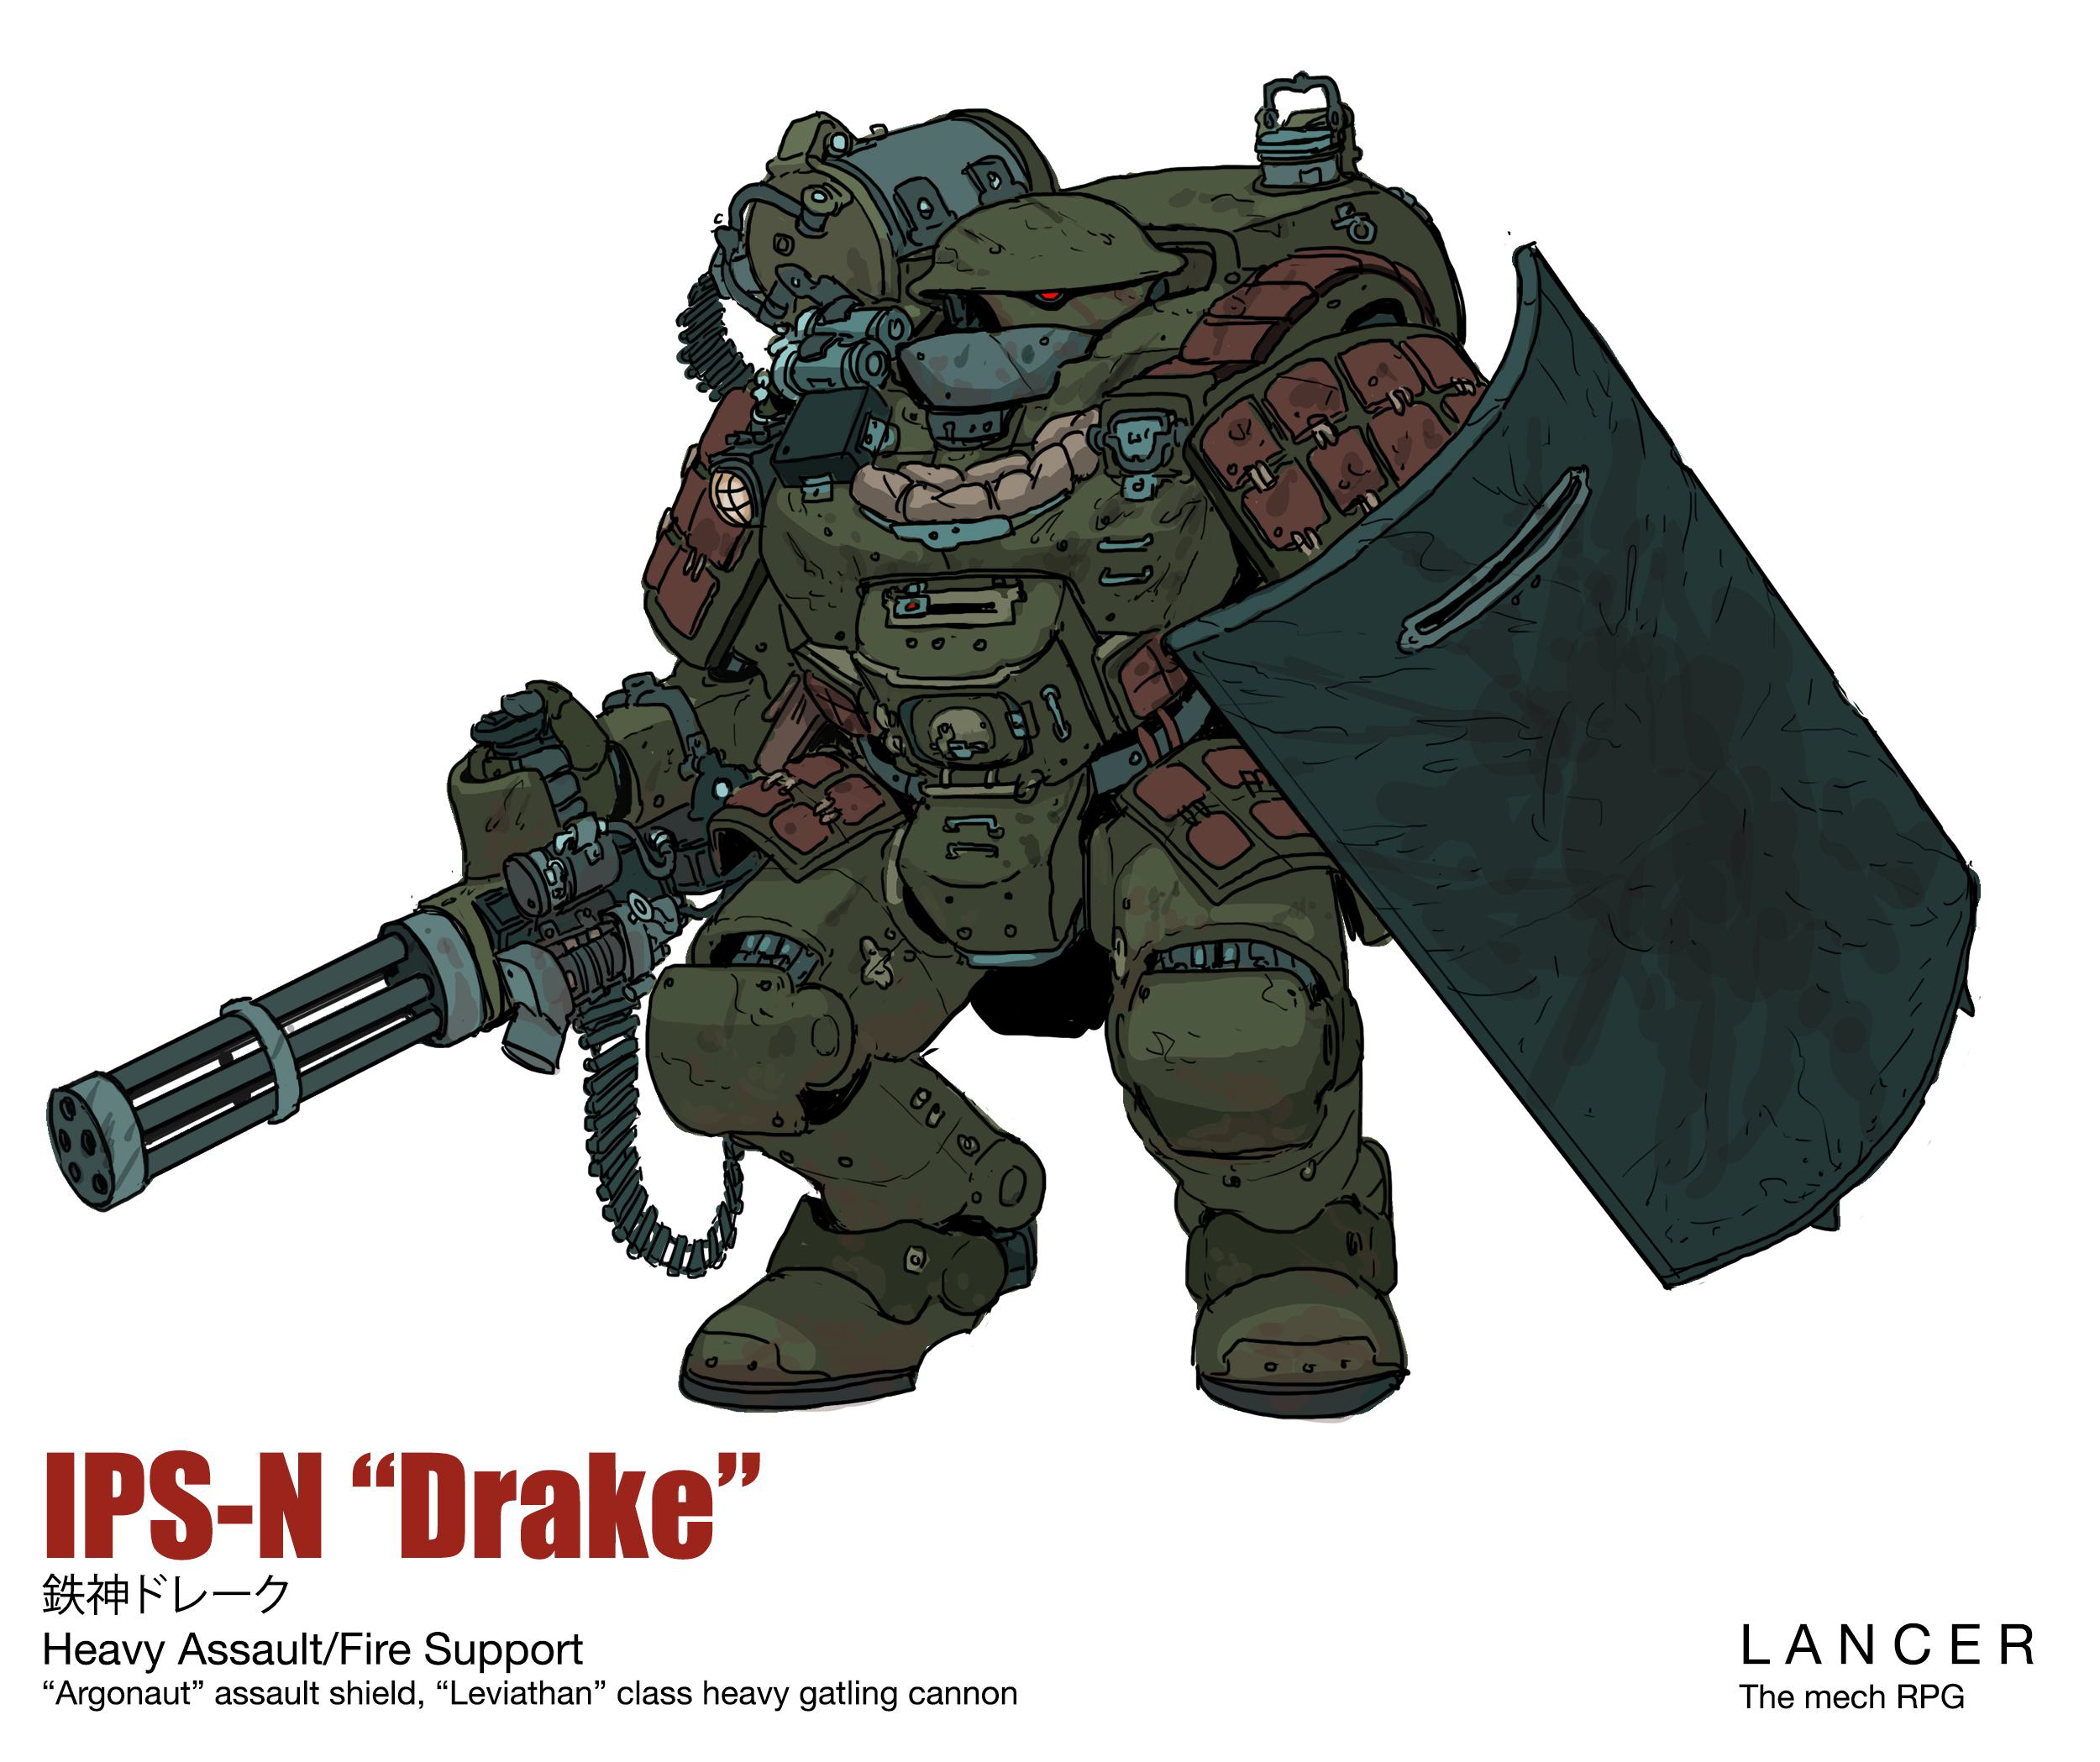
\includegraphics{Drake}
\end{center}

\begin{mech}{IPS-N}{Drake}

\fluff{The IPS-N DRAKE is the backbone of any proactive trade security/anti-piracy force and represents the manufacturers first foray into military-grade mechs. It is a massive frame, simian in appearance, built around a single-cast bulkhead sloped and reinforced to handle sustained incoming and outgoing fire.  

A dense heavily armored chassis, the standard IPS-N DRAKE fleet license includes a high-velocity, high-fragment assault cannon for suppressing and overwhelming their targets, and a heavy kinetic/ablative barrier shield for defense. More advanced models feature scaled-up weaponry and armor, including the notorious multi-barrel Leviathan cannon.
}

\begin{license}
\item Assault Cannon, Concussion Missiles
\item DRAKE FRAME, Aegis Shield Generator, IPS-N Argonaut Shield
\item Portable Bunker, Leviathan Heavy Assault Cannon
\end{license}


\frameBox
[hp = 8,
evasion = 6,
speed = 3,
heat cap = 5,
sensors = 10,
armor = 3,
e-defense = 6,
size = 2,
repair cap = 4,
tech attack = +0,
traits = {\textbf{Heavy Frame:} The Drake cannot be knocked back or prone by actors smaller than itself

\textbf{Blast Plating: }The Drake has resistance to damage from blast, line, and cone attacks

\textbf{Guardian:} Adjacent allied mechs can use the Drake for Light Cover

\textbf{Slow:} The Drake has +1 Difficulty on agility checks},
sp = 5,
mount one = main mount,
mount two = main mount,
mount three = heavy mount,
core system name = FORTRESS,
core system text = {},
core active text = {Protocol
When you activate this protocol, you plant your shield and deploy stabilizers, becoming more like a fortified emplacement than a mech. While this system is active, your mech is immobilized. Two line 2 sections of heavy cover unfold, drawn from your mech in any direction. Your mech grants and benefits from heavy cover for allied mechs while this system is active and also grants any allies that benefit from this cover its immunity to knockback, prone, and resistance to blast, line, and cone attacks. This system can be deactivated at the start of your turn but cannot be reactivated without more core power.}]


Assault Cannon
The IPS-N assault cannon is a deep-cooled autocannon, able to be fielded as a fixed weapon or manipulator-compatible platform. This autocannon can be fed by box-magazine or belt, is simple in its functionality, and is a mainstay among IPS-N chassis fleet orders. 

Main Cannon
1 heat (self), Overcharged
Range 8
1d6+2 Kinetic Damage

Concussion Missiles 
Main Launcher
Range 5
Knockback 2
1d3 explosive damage
Targets struck by these missiles must pass a hull check or become impaired until the end of their next turn.

Aegis Shield Generator
The Aegis is a portable electromagnetic shield generator, a way to establish a momentary safezone to withstand an incoming bombardment or environmental hazard.   

2 SP, Unique, Limited (1)
Shield, Deployable, Quick Action
Once planted in a free adjacent space, this size 1 generator creates a burst 2 zone around it until the end of the current scene. All allied targets at least partly covered by the zone gain +1 armor (up to 4). The generator has 10 HP but benefits from its own armor bonus, and deactivates once used up.

IPS-N Argonaut Shield

2 SP, Quick Action
As a quick action, this heavy over-arm shield can be used to protect an adjacent actor from incoming fire, giving them resistance to all damage as long as they stay adjacent to you. However, your mech takes the half that was resisted. The effect breaks if they break adjacency, and you must repeat this action to regain the effect.

Portable Bunker
A simple deployable, the “Portable Bunker” is actually a series of unfolding single-use printer sheets: flat-pack pouches of inert non-newtonian fluid that, when deployed, are triggered into a rigid structure capable of withstanding incredible force. 

2 SP, Limited (1)
Deployable, Quick Action
To activate this system, choose a clear 4x4 space adjacent to you and take a quick action. At the start of your next turn, this system unfolds into a fortified emplacement that grants heavy cover to anyone within the area from all directions, as long as they are fully covered by the area. Actors inside also have resistance to damage from blast, line, and cone attacks that originate from outside the bunker.

The bunker is open topped and can be entered and exited at will. If attacked the bunker has evasion 5 and 40 HP. It cannot be moved or deactivated once deployed.

Leviathan Heavy Assault Cannon
The Leviathan AC is a massive rotary autocannon, an enclosed multi-barrel automatic weapon fed by an external reservoir, usually dorsally mounted on the chassis carrying it. At its current chambering, the Leviathan should only be fired on automatic when absolutely necessary; IPS-N is currently working on a solution to meet the cannon’s needs remotely. IPS-N recommends outfitting willing squadmates with extra reservoirs, should their chassis have room to support it. 

Superheavy Cannon
2 heat (self)
Range 8
1d6 kinetic damage

Unlike other superheavies, this weapon can be fired as part of a skirmish action with its listed profile.
As a quick action, you can spin up this weapon’s barrels. While this weapon’s barrels are spinning, your mech is Slowed, but this weapon’s damage increases to 4d6+4 kinetic, it must be fired with a barrage action like a regular superheavy, and it gains Reliable 4. You can stop the spin-up as a free action at the start of your turn, but lose the increased damage until you spin the weapon up again.


\end{mech}


\subsection{IPS-N Lancaster}

                                         IPS-N LANCASTER  

The IPS-N LANCASTER is a mil-spec variant of an older IPS-N design, modernized and streamlined for  
military/operator use. The LANCASTER features multiple redundant systems and object/environment- 

interact projectors to facilitate pinpoint accuracy when engaging with delicate systems, damaged or intact.  
Commonly piloted by sapper and engineer-designate pilots in frontline support/specialist roles. 
 

                                                   License:
 
I. Restock Drone, Cable Winch System
 
II. LANCASTER FRAME, MULE harness, Sealant Spray
 
III. Plasma Cutter, Aceso Swarm
 

                                                LANCASTER 

  HP: 6          Evasion: 8                            Speed: 6           Heat Cap: 7        Sensors: 10 

  Armor: 1       E-Defense: 8                          Size: 2            Repair Cap: 10     Tech Attack:  
                                                                                             +0 

                                                   TRAITS: 

  Redundant Systems: Other friendly mechs of the Lancaster’s choice that are adjacent to it can spend  
  the Lancaster’s repairs as if they were their own
 
  Combat Repair: The Lancaster can spend a full action and 4 repairs in combat to repair a destroyed  
  mech, returning it to 1 structure and 1 HP 

                                             SYSTEM POINTS: 8 

                                                   MOUNTS: 

  Main/Aux Mount 

                                                CORE system 

                                                                                                            


                                                      Latch Drone  

  Known colloquially as a ‘Wingman’ drone, latch drones are companion drones carried upon and  
  deployed from a chassis. Pilots are advised against developing attachments to these drones, given their  
  high casualty rate.
 

   Integrated Mount:
 
  Latch Drone  
  Auxiliary Launcher
 
   Range 8
 
   Make a grit roll vs evasion 8 and target any friendly mech in range (still take cover and line of sight into  
   account). On hit, your target can spend up to 1 repair to heal.
 

  Active (requires 1 Core Power):
 
   Supercharger
 
   Quick action
 
  You fire your drone at a friendly mech in range, where it clamps onto the target. For the rest of this  
   scene, you take 1 heat at the start of your turn, but the targeted mech gains +1 Accuracy on all attacks  
   and checks, and is immune to the impaired, jammed, Slowed, and immobilized conditions. This effect  
   ends if you or the targeted mech is stunned or shut down. While this system is active, you cannot fire  
  your drone as a weapon (using the passive of this system). 

Restock Drone   

A simple, reliable, and sturdy drone mounting a printer, a restock drone allows for limited logistic capability  
through autosalvage: the bulk of the drone is RawMat, a generalized mix of silicates and metallic materials  
meant to be processed for high-yield printing. Pilots often call restock drones a “mech snack”.    

2 SP, Limited (2)  

Drone  
As a quick action, you can set this drone down in any adjacent space. After your turn ends, the  
drone primes. Any allied mech that moves adjacent to the drone can activate it as an interaction.  
That mech can then cool 1d6 heat, reload all weapons with the loading tag, and end one  
condition affecting it. The drone is then consumed, deactivating and disintegrating.
 

Cable Winch System   

A winch system consists of a spool of nanocarbon-weave cable mounted externally, and recovery  
subroutine software uploaded onto the recovery mech’s datamind.   

1 SP  

Quick action  
As a quick action, you can attach the cables to an adjacent mech. If the mech is shut down,  
stunned, or a willing target, this action is automatically successful, otherwise it can make a hull  
check to resist this effect. Once attached, your mech and the attached mech cannot move more  
than 5 range away from each other. One mech can tow the other, but is Slowed while doing so,  
and must successfully pass a hull check to do so. Any mech can make a successful melee or  
improvised attack to remove the cables (removed on a hit, the cables have evasion 10). The  

                                                                                                                      


cables can also be attached to the environment or any object. They are 10 length when used this  
way and can take a combined size of 6 in strain if using them to climb, etc, before they break.
 

MULE harness  
The Multiple User, Light Entanglement harness is a mass-produced version of a common battlefield  
modification that allows friendly soldiers to ride along on friendly chassis. Some systems are large and  
sturdy enough to allow for smaller chassis to accompany larger chassis; these are typically employed in  
High Altitude, Low Orbit insertions to reduce radar signatures.  

2 SP, Unique  
Your mech has mounts, straps, and hard points built to carry a total number of actors whose   
total size is less than your own (so size 1 = 1 size 1 actor, two size 1/2 actors). Actors of your  
choice that are adjacent to you can spend a quick action to mount your mech. While mounting  
your mech, they occupy your mechs’s space, move when you move and benefit from light cover.  
Any area of effect attacks that target your space will also target your rider. If your mech is  
knocked prone or is destroyed, they fall off into an adjacent space. They can dismount by  
moving normally off your mech any time.  

Sealant Spray  

2 SP  
Quick Action  

This system can be used on any actor or free space within range 5 and line of sight. It has  
different effects depending on what it is used on
 
         	Hostile actor: Make a ranged attack vs the target. On hit, the target is Slowed until the  
         start of your next turn but immediately ends any Burn affecting them.
 
         	Empty space: This creates a blast 2 area around the targeted space. The area becomes  
         difficult terrain for the rest of this scene and this puts out any fires in the area.
 
         Allied actor: 	  Your target is Slowed until the start of your next turn but can immediately  
         end any Burn effecting them.
 

Plasma Cutter
 

Plasma cutters were tools first, simple blades built to toggle and sustain a plasma sheath to make cutting  
metal easier for its user. Repeated ad-hoc use of cutters as a personal defense weapon to repel pirate  

boarding actions convinced IPS-N of the need for a mil-spec variant of the civilian tool. They developed the  
Cutter, now in its second generation. The Cutter MkII is hard-lined into the mech’s power core, with a port  
to attach power packs in case of cord severance. The cutting edge can be shortened to a knife variant, but  

is most popular in its “cutlass” option, a middling length variant that allows for a balance of reach and  

maneuverability in close quarters.    
 

Auxiliary Melee
 
1 heat (self)
 
Threat 1
 
1 energy damage +1 heat + Burn 1
 
Against objects and the environment, the cutter deals 10 AP energy damage
 

                                                                                                                     


Aceso Swarm  

The IPS-N Aceso Swarm system is a useful triage measure to address scoring and minor mechanical  
damage that results from combat engagements or negative environmental interaction. Due its low  

processor demand, an Aceso Swarm can be controlled by even a comp/con unit; this allows the pilot to  
concentrate on more complex repairs or immediate threat neutralization.    

3 SP, Unique  
Drone, Quick action  
Once per round, as a quick action at any point during your turn, your mech takes 1d6 heat and  
one other mech of your choice in your sensor range can spend 1 repair to heal.   


\section{IPS-N Nelson}

\begin{mech}{IPS-N}{Nelson}

\fluff{The IPS-N NELSON brings the close-quarters doctrine espoused by ISP-N to its most pure form. The NELSON is built to brawl in environments too volatile for firearms or when ordnance has been exhausted.

With its functional size, the NELSON can attack fast while remaining a difficult target to track. Layers of fractal-fold BULWARK plating allows for ceramic-analogous carbon flaking, effectively nulling the impact of incoming solid-state fire by dispersing kinetic energy across a rounded hull. This null-k plating protects the pilot from impact trauma, allowing for sustained combat efficacy in high-trade scenarios.

The NELSON is an iconic IPS-N chassis, known across the galaxy as the FRAME of choice for the Albatross, the Cosmopolitan interstellar anti-piracy agency. Their distinctive white, gold, and red livery and mastery of the war pike -- as well as seeming agelessness due to time dilation -- has won both the Albatross and the NELSON a venerated place in Diasporan lore -- and secured the Albatross an endorsement contract with IPS-N in perpetuity.}

\begin{license}
\item War Pike, Bulwark Mods
\item NELSON FRAME, Thermal Charge, Armor Lock System
\item Power knuckles, RAMJET
\end{license}

\frameBox
[hp = 8,
evasion = 10,
speed = 5,
heat cap = 6,
sensors = 10,
armor = 0,
e-defense = 8,
size = 1,
repair cap = 5,
tech attack = +0,
traits = {\textbf{Momentum:} After making the boost action, the next melee attack from the Nelson deals +1d6 bonus damage on hit

\textbf{Skirmisher:} After making any attack, the Nelson can move 1 in any direction. This movement doesn’t provoke reactions, ignores engagement, and doesn’t count against its movement for the turn. It can’t make this move if immobilized or slowed.},
sp = 6,
mount one = flex mount,
mount two = main/aux mount,
core system name = Perpetual Momentum Drive,
core system text = {IPS-N’s PMD exploits fighter-tier nearlight spooling to conserve and sustain a passive .000001LS charge, able to be dumped into extant boost systems at the pilot’s command. The chassis fielding this system must be heavily adapted through strengthening joints, limbs, and installing a k-comp crash couch to protect the pilot from sudden g force and shear.},
core active name = Spool up PMD,
core active text = {Protocol
   Once activated, this system remains active until the rest of the current scene. While its active, the free movement from the Nelson’s Skirmisher trait increases to 4.}]

War Pike

A War Pike is a simple weapon. A long haft, topped with a dense, slim point, meant to puncture armor. Derivative of a mining pylon, the modern war pike is a sturdy, balanced, and reliable weapon, perfect for a charge.

Main Melee
Thrown 5, Threat 3, Knockback 1
1d6 kinetic damage


Bulwark Mods

A mark of pride for IPS-N, all proprietary mech cores feature IPS-N’s QuickMod system, a modular, legacy- compatible system of joints, hardpoints, and internal slots that make installing upgrades simple.

1 SP
Your mech has extended or armored arms or legs, redundant motor systems, or is otherwise reinforced for harsh terrain. Your mech ignores difficult terrain.


Armor Lock System

IPS-N’s Armor Lock System is a total-body modification for a mech core that provides additional chassis stability when pilots are faced with a situation that puts their core under greater-than-anticipated stress.

1 SP, Unique
2 heat (self)

When you take the Brace reaction, you can activate this system. Until the end of your following turn, enemy attacks targeting you are made with 1 additional Difficulty, you can’t fail agility or hull checks, be knocked back, grappled, knocked prone, or moved by any external force smaller than size 5. You end any grapples currently affecting you.


Thermal Charge

Pilots have long made this popular modification to their pikes. Now, IPS-N is offering these pilots’ modifications as a licensed and quality-tested suite for pan-galactic printing. A pike modified with a charge -- often colloquially called a “Fire Pike”-- is a simple plasma projector integrated into war pike, tuned to project a plasma sheath over the pike’s head.

2 SP
Mod
\Limited{3}

This mod can only be applied to a melee weapon. As a free action when you hit with any melee attack, you may spend a charge of this system to activate the shaped charge on your weapon and deal +1d6 bonus explosive damage.

Power Knuckles

A simple weapon system, IPS-N’s power knuckles are a popular modification for pilots of CQB mech cores. Whether as shaped studs, hyperdense knuckles, or a series of magnetically-accelerated micro-rams, power knuckles amplify the already incredible hitting power of a mech core.

Auxiliary Melee

Threat 1
1d3+1 explosive damage

On a Critical Hit, your target must pass a hull check or be knocked prone

RAMJET
Air. Air and momentum. There’s a threshold that veteran Nelson pilots know well, the Point of Endless Momentum. When you get moving fast enough, in the right atmosphere, the air itself feeds into auxiliary ports on the chassis, compressing, howling out like a demon’s angry scream. The Point of Endless Momentum is a giant’s hand on your chest and a god’s chariot under your feet and you feel like you can outrun light itself and there’s nothing else like it.

3 SP, Unique

Protocol
2 heat (self)

Until the start of your next turn, your mech gains +2 speed when boosting and its melee attacks (including rams, grapples, etc) gain knock back +2. However, your mech must move its maximum speed each time it moves and can only move in straight lines (it can stop if it would collide with an obstacle or enemy, and it can change direction between movements).

\end{mech}


% \subsection{IPS-N Raleigh}

% \begin{center}
%     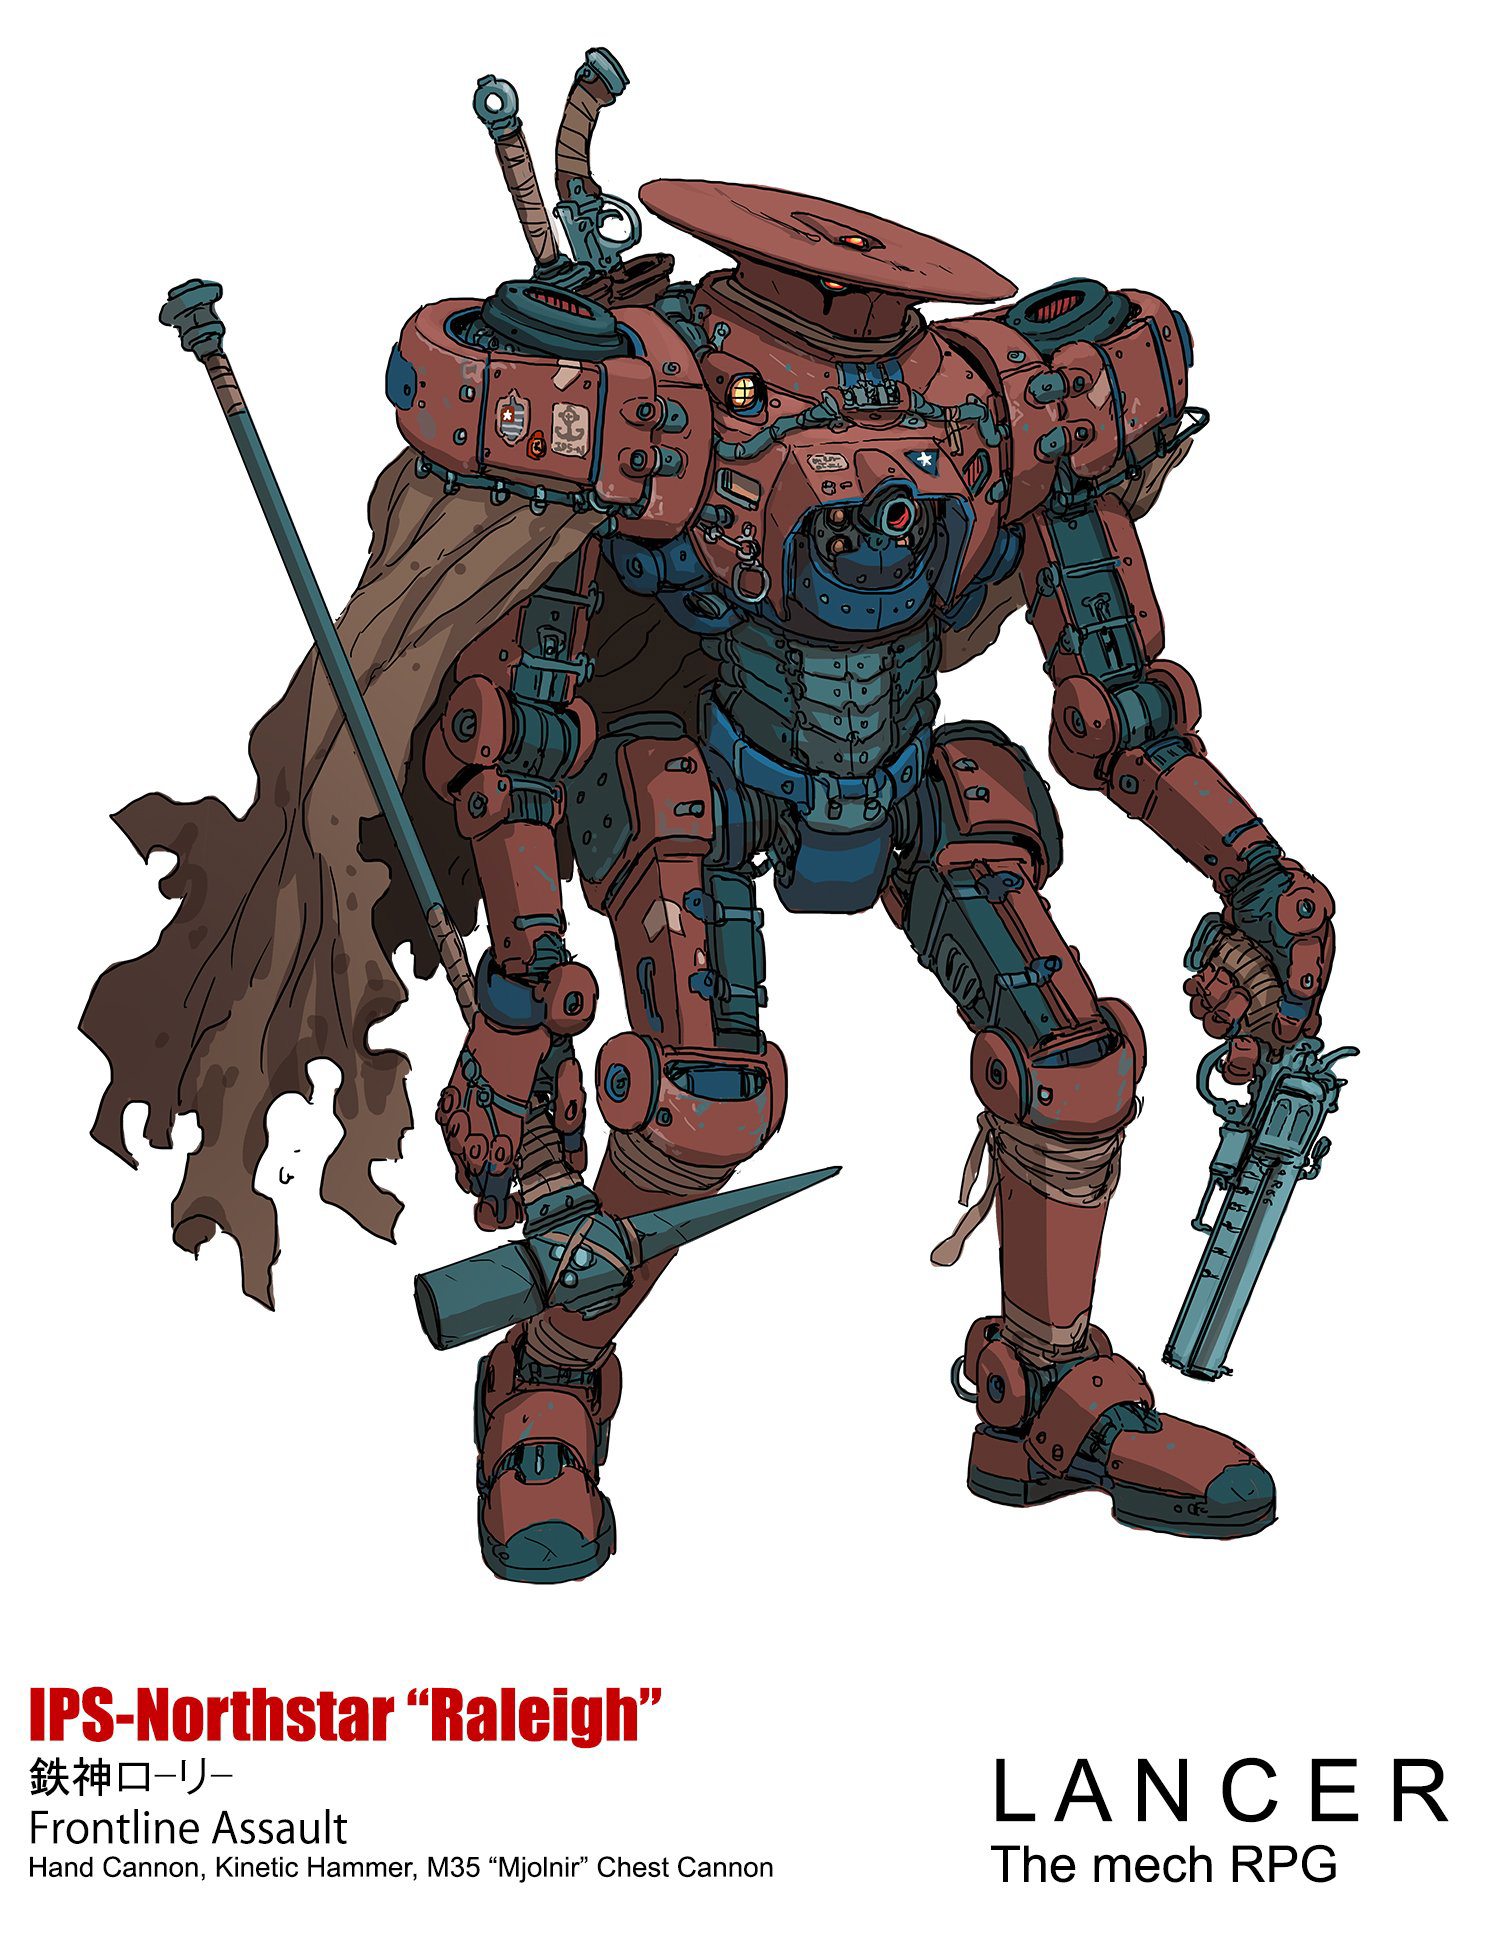
\includegraphics{Raleigh}
% \end{center}

\begin{mech}{IPS-N}{Raleigh}

\fluff{The IPS-N RALEIGH, more so than any other mech in IPS-N's core line, is meant to meet any enemy, any where, in any combat scenario. The RALEIGH is an all-rounder build that trends towards the midrange. It is commonly outfitted with an auxiliary hand cannon for ranged capability, a massive hammer to deal with anything that gets close, and the iconic, chest-mounted MJOLNIR cannon.}

\begin{license}
\item Hand Cannon, Breaching Charges
\item RALEIGH FRAME, ROLAND Chamber, Bolt Thrower
\item UNCLE class NHP, Kinetic Hammer
\end{license}

\frameBox
[hp = 10,
evasion = 8,
speed = 4,
heat cap = 5,
sensors = 10,
armor = 1,
e-defense = 8,
size = 1,
repair cap = 5,
tech attack = +0,
traits = {\textbf{Full Metal Jacket:} If the Raleigh makes no attack rolls during its turn, it can re-load all weapons with the loading tag at the end of its turn as a free action.

\textbf{Shielded Magazines:} The Raleigh can still make ranged attacks if it is Jammed.},
sp = 5,
mount one = aux/aux mount,
mount two = flex mount,
mount three = heavy mount,
core system name = IPS-N M35 `Mjolnir' cannon,
core system text = {IPS-N's M35 MJOLNIR cannon is a carryover from Northstar's WATCHMAN line of defensive weapons, reworked for frontline combat. The MJOLNIR is a hard-mount, multi-barrel auxiliary cannon that uses magnetic acceleration to fire stacks of airburst projectiles at its target. It is an impulse weapon, a system tied to a pilot's second-tier neural processes as dictated and coached by their partner Comp/Con or NHP; even in death, a pilot's MJOLNIR will continue to identify and attack hostile targets until total systemic failure. For this reason, the MJOLNIR is often referred to as a deadgun, one of many such weapons common among CQB-oriented pilots.

Integrated Mount:
M35
Main CQB
Range 5, Threat 3
4 kinetic damage},
core active name = Thunder God,
core active text = {Protocol

Until the end of the current challenge, if you didn't fire your M35 on your turn, it gains 2 more rounds in the chamber at the end your turn (you can use a d6 to track this). It starts with 0 rounds in the chamber. When you next fire the weapon, it fires all chambers, for 4 damage per chamber. The M35 has six chambers, for a maximum of 24 damage. If 4 or more chambers are fired at once, this weapon gains the AP tag and any target struck must pass a hull check or be knocked prone.}]


Hand Cannon
The IPS-N HAND CANNON is a licensed version of GMS's Pattern I Pistol, chambered for a heavier caliber of round. This modification requires a change from the belt-fed system of the P1P to a magazine-based system, limiting the number of rounds that a mech can load at a time.

Auxiliary CQB
Loading, Reliable 1
Range 5, Threat 3
1d6 damage

Breaching Charge
A breach/blast charge is simply a shaped, milspec pattern of IPS-N's generalist/civilian blasting charge, meant to crack asteroids. The IPS-N BB features a far more pure blend of high explosives designed to cause massive traumatic damage to mechs and other hardened structures.

2 SP, Limited (2)
Grenade, Mine
If thrown as a quick action, the charge explodes on impact. If planted as a mine, it can be detonated as another quick action by whoever planted it (or detonates normally when a target moves adjacent). The charge deals 2d6 Energy damage to targets in a burst 1 area around the charge. Targets can pass an agility check to reduce this damage by half. Against objects, this charge does 10 AP kinetic damage.

ROLAND Chamber
Packed into sealed, self-contained cylinders, IPS-N's ROLAND rounds are heavy shells purpose-built for any kinetic weapon that can accept cylindrical magazines. Packed with a non-O2 dependent accelerant, ROLAND Chambers can be used to reliably send air-or-impact burst shells downrange.

For use in outdoor or Certain-Kill environments; use extreme caution when firing in pressurized spaces.

2 SP, Unique
When you reload, your very next attack deals +1d6 bonus damage as explosive damage and targets affected by this bonus damage must pass a hull check with 1 difficulty or be knocked prone.

Bolt Thrower
IPS-N's bolt thrower is a milspec variant of a civilian mining tool. A bolt thrower fires self-propelled explosive bolts that can be triggered manually, on a timer, on impact, on designated-depth penetration, on proximity, on on some combination of any allowable parameter.

Heavy Rifle
Loading, Range 8
Reliable 2
2d6 kinetic + 1d6 explosive damage

UNCLE-class NHP
IPS-N's UNCLE NHP is the result of the DARKSTAR Program, an NHP think tank funded by IPS-N's Administrator Partnership. UNCLE is a pocket-AI, meant to be bound to a weapon system and assist its owner in peak-efficiency operation. UNCLE AI's are currently available only as a beta system and, as such, owners are expected to accept all pushed updates; IPS-N waives culpability for any sub-optimal performance of UNCLE systems not kept current via Omninet updater.
UNCLE NHPs are (perhaps unfairly) regarded as lesser compared to their compatriots and their inferiority complexes tend to display themselves as unstable personalities.

3 SP, Unique
Mod
Choose 1 weapon - The weapon and its associate systems gain an NHP that has control over that specific weapon. This is not a full AI and can't control your mech or become unshackled (and doesn't have the AI tag).

It can attack by itself once on your turn as a free action, using the mech's attack bonuses but with +2 Difficulty. It can't fire a weapon that has already been fired this turn, and if you fire a weapon with UNCLE you cannot use it until the start of your next turn.

Kinetic Hammer
A Kinetic Hammer is, in the trend of IPS-N weapons, a simple tool. A supermassive, shaped head fused to a long haft, the Hammer impacts with enough force to create massively traumatic pressure waves upon landing a successful blow.

Heavy Melee
Reliable 3
Threat 1
2d6+2 kinetic damage



\end{mech}


\section{IPS-N Tortuga}

\begin{center}
    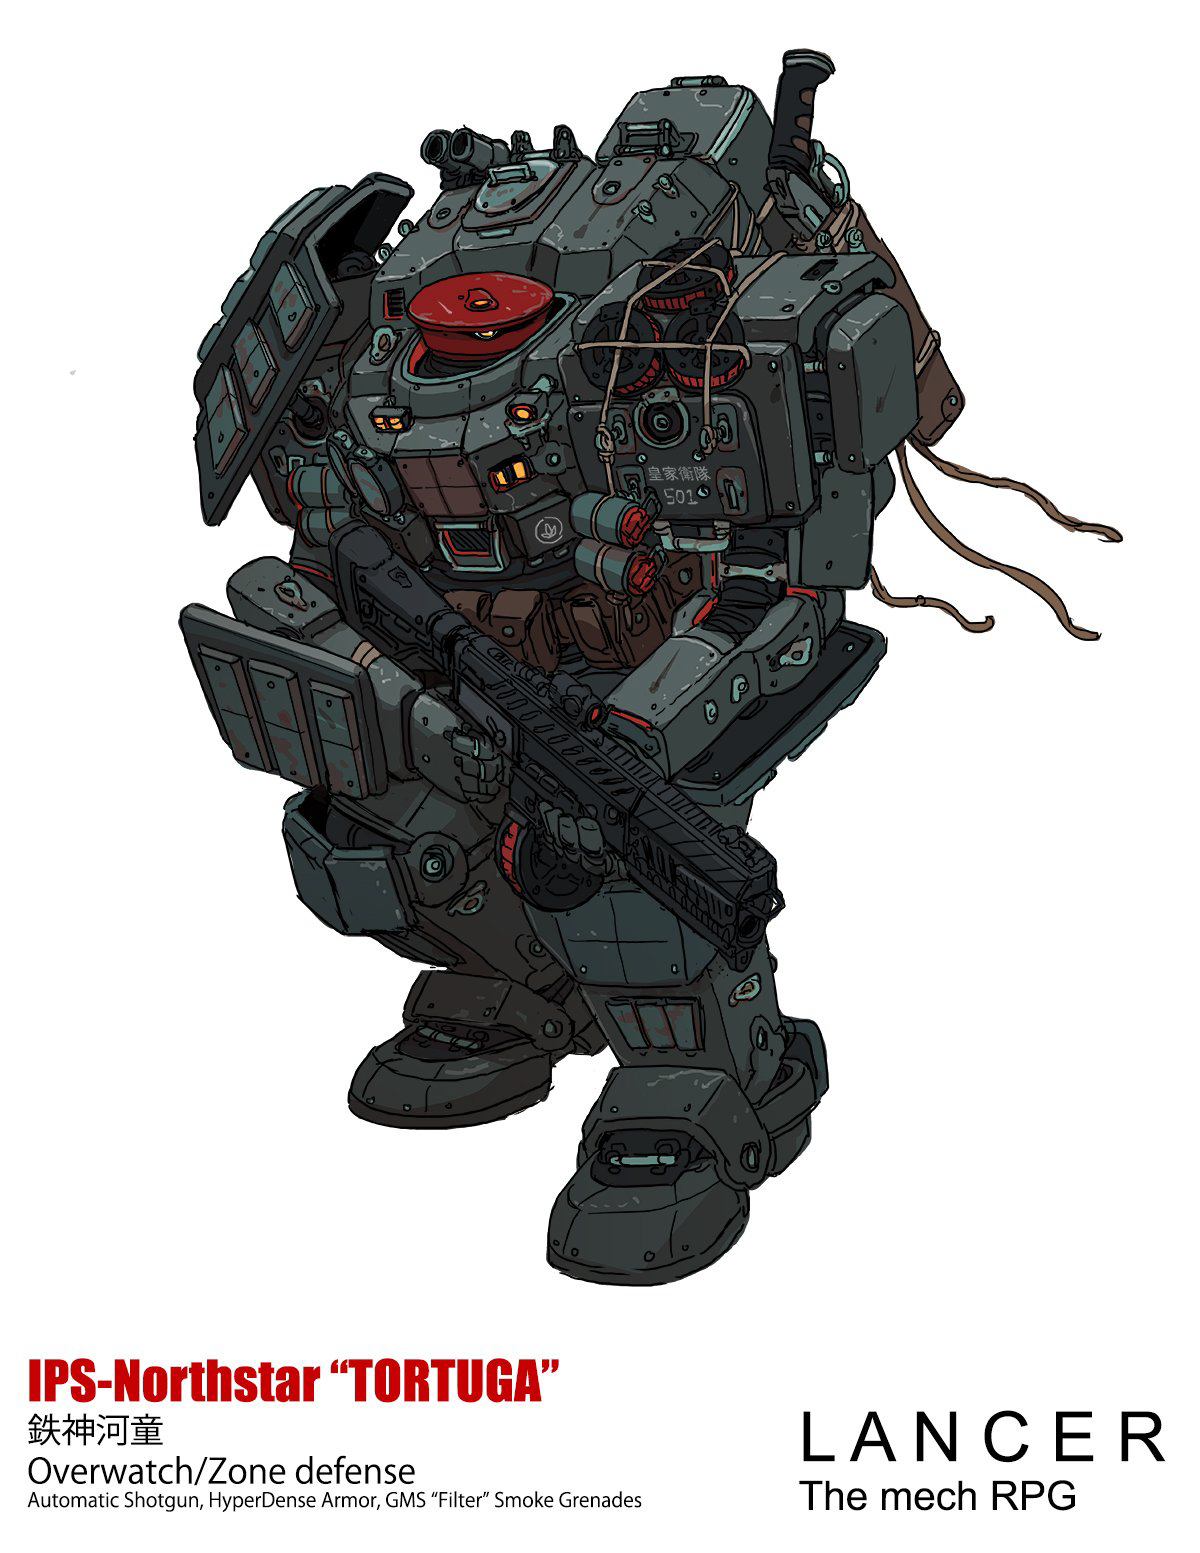
\includegraphics{Tortuga}
\end{center}

\begin{mech}{IPS-N}{Tortuga}

\fluff{The TORTUGA is IPS-N’s short-to-medium range core-line mech. Conceived, tested, and perfected in the void of deep trade space, the TORTUGA is made to breach and clear the spinal columns of capital ships, carriers, and hostile stations. The TORTUGA is built to occupy space, filling hallways with its angular bulk. It defends just as effectively as it attacks, often used in a battering-ram role by boarding parties and ship/stationboard marines. Conversely, the Tortuga is often employed in a defensive posture by marines seeking to repel boarding parties, often using its ablative brachial structures to shield troopers from incoming fire.}

\begin{license}
\item Automatic Shotgun, Siege Ram
\item TORTUGA FRAME, Throughbolt Rounds, Daisy Cutter
\item Pneumatic Hammer, Hyper Dense Armor
\end{license}

\frameBox
[hp = 10,
evasion = 6,
speed = 3,
heat cap = 6,
sensors = 15,
armor = 2,
e-defense = 10,
size = 2,
repair cap = 6,
tech attack = +1,
traits = {\textbf{REFLEX:} The Tortuga gets +1 Accuracy to all overwatch attacks

\textbf{Guardian:} Allied actors adjacent to the Tortuga gain light cover },
sp = 6,
mount one = main mount,
mount two = heavy mount,
core system name = SENTINEL,
core system text = {IPS-N security teams are no strangers to the danger of ship-to-ship or ship-to-station boarding actions. Tight corridors, unstable gravity, dark environments, hard vacuum, and the dual threat of organic and inorganic opposition forces make boarding actions some of the most deadly engagements (by percentage) that one could participate in -- the winning side, according to IPS-N’s internal metrics, should expect at least 30\% casualties on average.

To lessen the cognitive burden of pilots and any NHPs or comp/cons they have installed in their chassis, IPS-N developed the SENTINEL co-pilot subsentient partition. The Sentinel is a simple subsentient: a flash-homunculus of an aggregate-intelligence compiled through thousands of after-action reports from boarding actions, debriefings, and volunteer donors. Not a true AI, nor an NHP, the SENTINEL is a robust tactical program similar to a smart weapon, though without the need to cycle it presents certain tactical advantages -- namely, the ability for limited learning and best-guess predictive capabilities alongside its pilot. SENTINELs are largely plain in their personalities, such that they develop, and are a favorite of pilots for their no-nonsense attitude and crisp, efficient counsel. 

The SENTINEL is currently under review by a joint USB/UDoJ-HR committee, but no formal stay on production has yet been issued.},
core active name = Hyper-reflex mode,
core active text = {Protocol

For the rest of this combat, your threat with ranged weapons increases to 5 if it was less than 5. You can make one additional overwatch attack between your turns, and any target struck by your overwatch attacks is immediately immobilized until the start of its next turn.}]


Automatic Shotgun
The IPS-N Deck-Sweeper Automatic Shotgun is a belt-fed scattergun, a favorite of marine pilots aboard stations and capital ships. It’s operation is simple and straightforward: charge, point, and fire. The single-barrel constriction allows for pneumatic absorption, dampening the effect of its incredible recoil, and its belt-fed action accepts many types of shot-and-FRAME ammunition. 
The DSAS is a mainstay among IPS-N licensed pilots.   

Main CQB
Inaccurate
Range 3, Threat 3
2d6 Kinetic Damage

Siege Ram
The Siege Ram is another holdover from IPS-N’s pre-merger days. When Bulkheads slam closed and there is a need to get them open, marine pilots mount a siege ram to get the job done. Heavy, dumb, and unbreakable, the Siege Ram is the universal key. Carried in-hand by a qualified chassis, the IPS-N Siege Ram is a solid metal beam with a wedge tip, meant to be slammed into the seam of a sealed bulkhead door and driven home, cracking open ships and stations like a can.  

2 SP, Unique

Your ram attacks deal 1d3 kinetic damage on hit. Against stationary objects, deployed cover, terrain, walls, or obstacles, your ram attacks instead deal 10 AP kinetic damage.

Throughbolt Rounds
Throughbolt Rounds are a proprietary IPS-N invention. Throughbolts are Tungsten-jacketed, uranium core rounds with projection-activated plasma sheaths. When fired, the rounds ignite and project a superheated cone of plasma before them, creating a miniature lance effect that ensures multiple-target penetration through soft and hard surfaces.  

2 SP
Mod
Choose 1 CQB, cannon, or rifle weapon. When you fire this weapon, draw a line 3 spaces long from your mech, then measure its original range from the end of this line as though the attack was fired from that position (also measure cover and line of sight from this new position for the rest of the attack). This line can easily punch through walls or other barriers. Any targets hit by this line are also hit by the attack. The attack cannot change directions after being fired.

Daisy Cutter
The Daisy Cutter is an effective, if outdated, weapon system for which many marine pilots still place print requisitions. The Daisy Cutter is, essentially, a massive shotgun: the pilot loads a shaped charge into the breech of the Cutter, drops a packed sabot down the barrel, aims, and fires a mixed hellfire cloud of flechette darts, bearings, and ignited magnesium strips, clearing any deck it’s been fired on. 

Heavy CQB
Limited (1)
Cone 5
3d6 kinetic damage. 
The blast cloud from firing this weapon lingers until the end of your next turn, providing light cover to any actor in the affected area.

Pneumatic Hammer
Colloquially known as a ‘pilebunker’, built originally from blast mining equipment, the pneumatic hammer has been refined into a widely feared weapon - a solid-core cylinder cocked and locked in place by a miniaturized gravity well. When fired, the cylinder is propelled forward by a charge of superheated plasma through a cannon-like shaft, creating enormous kinetic force. Without proper reinforcement, the power created by this weapon will literally tear its wielder’s arm off.

Main Melee
Loading
Threat 1
1d3+5 kinetic damage
On a Critical Hit with this weapon, your target must pass a hull check or be stunned until the end of its next turn.

Hyper Dense Armor
IPS-N HyperDense Armor is built for use in space. As the name implies, the HyperDense system is forged without respect to the gravitational constraints mechs may face down a gravity well; many pilots flying cores equipped with HyperDense armor are shocked to experience the difference in piloting their mechs down a well versus in the null-gravity of space. 

3 SP
Unique, Protocol, 2 heat (self)
You may activate or deactivate this armor system’s activation protocols at the start of your turn. While active, it hardens into a shimmering, reflective surface and offers unparalleled protection, granting you resistance to all damage from attacks further away from range 5 of your mech. However, your mech is Slowed while it is active. 


\end{mech}


\section{IPS-N Vlad}

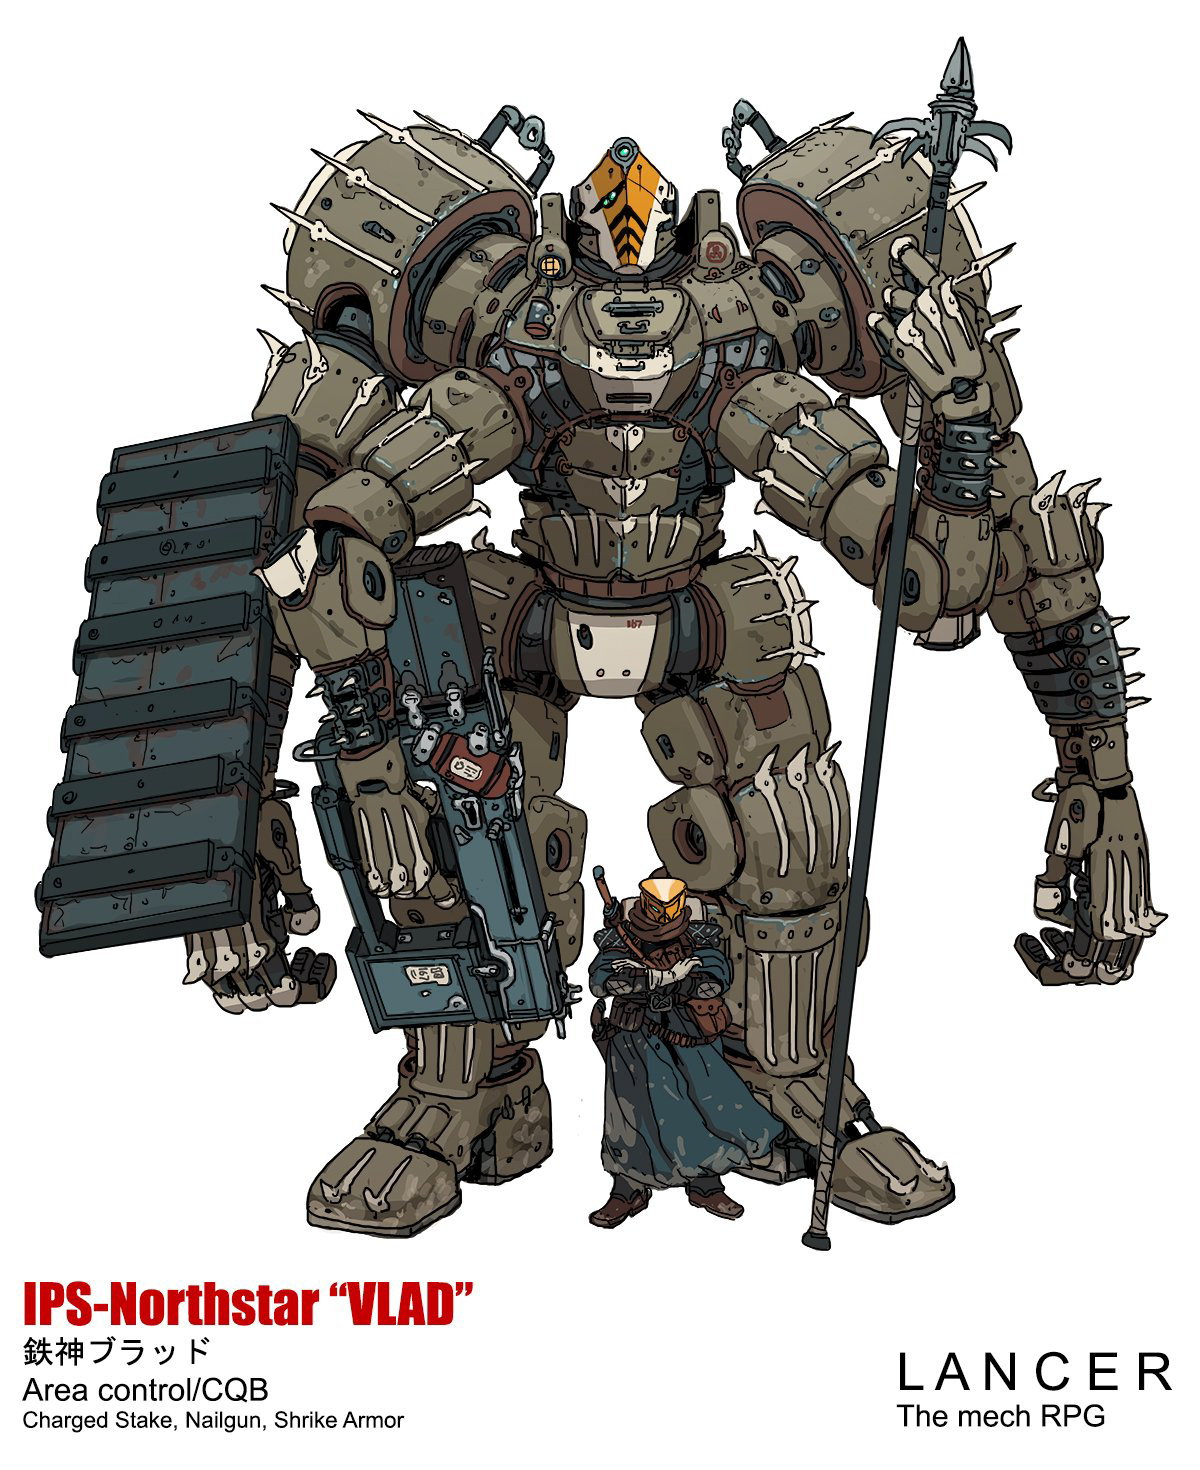
\includegraphics{Vlad}

                                                     IPS-N VLAD

The IPS-N VLAD is a variant of the IPS-N NELSON, built to handle hardened targets that would present

strategic difficulty for the NELSON platform. The VLAD features a suite of myth-inspired weaponry and
heavy armor and is meant to take a frontline role, absorbing fire from dangerous targets in order to protect
its allies while lining up the perfect shot.




                                                      License:

I. Snare Trap, Impact Lance

II. VLAD FRAME, Nail Gun, Caltrop Launcher

III. Combat Drill, Charged Stake


                                                       VLAD

  HP: 10          Evasion: 8                              Speed: 4            Heat Cap: 4         Sensors: 5

  Armor: 2        E-Defense: 8                            Size: 1             Repair Cap: 4       Tech Attack:
                                                                                                  +0

                                                      TRAITS:

  Dismemberment: When the Vlad successfully immobilizes a target, that target is also Shredded for the
  same duration

  Shrike Armor: When the Vlad is attacked by any actor within range 3, the attacker takes 1 AP kinetic
  damage before they attack

                                                SYSTEM POINTS: 5

                                                      MOUNTS:

  Flex Mount                          Main Mount                               Heavy Mount

                                                   CORE system

                                                    Shrike Armor
  A nod to the pre-Fall namesake of the VLAD, Shrike armor plating bristles with shaped spikes, hardened
  with chromium/tungsten alloy tips. Strategic studding places Shrike tips in high-likelihood kinetic
  encounter areas: gauntlet covers, manipulator joint covers, shoulder plating, and so on. Primarily a
  defensive modification, Shrike armor is uncommon among Coreside pilots, and seen as a mark of
  underdeveloped -- if terrifying - tactics.

  Active (requires 1 Core Power):
  Tormentor spines
  Protocol
  Until the end of the current challenge, you gain resistance to all damage from within range 3, and your
  damage from this mech’s Shrike Armor trait increases to 3 AP kinetic damage.

Snare Trap
The IPS-N WEBJAW Explosively-Accelerated Filament system is a deployable all-theater perimeter
defense system designed to arrest hostile movement in pre-determined kill-corridors. Deployable by hand
or launch tube, the WEBJAW EAF system consists of a cluster of filament anchors scattered across an
area. When triggered remotely or by a series of programmable physical, electronic, or chemical triggers, the
anchors target and fire at the triggering foe, embedding hard-tip barbs deep inside both hard and soft
targets. The barbs, anchored to their bases by arachnosilk-analog filament, immobilize and entangle the
target.




1 SP
Mine, Limited 1

This trap triggers when any actor passes directly over it. The target must pass a hull check or
take 2d6 AP kinetic damage and become immobilized. Once triggered, the trap becomes an
object with 10 HP and 5 evasion, and immobilizes its target as long as it is not destroyed.


Impact Lance
The Impact Lance is a milspec variant of a common mining tool: the single-use, proximal-distance chemical
survey laser. IPS-N’s military variant mounts a series of Impact Lances on a brachial or thoracic carriages,
leaving a chassis’ manipulators free to field other weapons and systems; the Lance can be wired directly
into a chassis’ core, or charged with single-use chemical batteries.

The lances fire for a microsecond, burning through their stored charge in a milisolar burst of light that stabs
out in a tight, pulsed beam capable of searing through multiple meters of hardened bulkhead.

Main Melee

Threat 2

1d6 energy damage

This weapon attacks in a line drawn between its target and your mech, attacking all other actors
in between, but deals +1 heat to your mech for each target hit past the first


IPS-N “Impaler” Nailgun

The milspec Nailgun utilizes non-combustible, sabot-jacketed two-stage macroflechettes to pierce even

the most substantial of armor. First catapulted from its launcher, the macroflechette’s sabot disengages on
approach to its target, triggering a second stage where internal propulsion drives the macroflechette
forward with incredible velocity. Against soft targets, over-penetration is certain: IPS-N advises pilots

employ this weapon platform only when the area behind the target is clear of allies and/or noncombatants.

Main CQB

1 heat (self)

Range 8, Threat 3

1d6 kinetic damage

On a Critical Hit, the target of this attack must pass a hull check or be immobilized until the end
of its next turn


Caltrop Launcher
A wicked anti-organic, anti-vehicle, proximity denial system, chassis-mounted caltrops are fired in great
clouds of shimmering metal (or deployed in long swathes) to blanket an area.

IPS-N’s HX-CAL caltrop system adds small, shaped explosives to the mix of hardened pyramids.

1 SP, Unique

Quick Action

When this system is activated, your mech targets a free space within range 5 and blankets a
blast 1 area centered on that space with explosive caltrops. That area becomes difficult terrain,




and mechs moving across the space (voluntarily or otherwise) take 1 AP explosive damage for
each space they move.


Combat Drill

The IPS-N combat drill is a brutal close combat weapon, powered by a massive catalyst pack mounted
externally on a mech core. The drill is tipped with micro-plasmatic projectors designed to pre-treat the

target to ensure bit purchase and facilitate drill penetration.

Superheavy Melee

Overcharged, AP

Threat 1

3d6 kinetic + 1d6 energy


Charged Stake


Built from gear meant originally for blast mining, this enormous, improvised system is loaded and cocked
prior to embark into a specially primed chamber. It is designed to penetrate and immobilize hardened

targets, then send powerful, vaporizing charges into its vulnerable internal systems.

2 SP


Full Action
This brutal system can be used against any adjacent target. That target must pass a hull check
with 1 difficulty or take 2d6 energy damage damage and become immobilized and impaled. At
the end of each of its turns, the target can repeat this check to end the effect on itself, otherwise
it takes 3 AP energy damage and remains immobilized until it makes the check successfully. Only
one target can be immobilized by this system at once, but it can be picked up as a quick action.




